\section{Data serialization}\label{sec:dsdl_data_serialization}

\subsection{General principles}

A serialized data structure of type $A$ is an ordered set of data fields joined together into a bit string
according to the DSDL definition of the data structure $A$.
The ordering of the fields follows that of the data structure definition.

Serialized bit strings do not have any implicit data entities such as padding or headers.
Data type developers are advised\footnote{But not required.} to manually align fields at
byte boundaries using the void data types
in order to simplify data layouts and improve the performance of serialization and deserialization routines.

Serialized fields follow the little-endian byte order\footnote{Least-significant byte (LSB) first.}.
One byte is assumed to contain exactly eight bits.
Bits are filled from the most significant bit to the least significant bit,
i.e., the most significant bit has the index 0.

Serialized data structures must be padded upon completion to one byte,
with the pad bits set to zero.
Lower layers of the protocol may also add additional padding as
necessary\footnote{More on this in the chapter \ref{sec:transport_layer}.};
however, the rules and patterns of such padding fall out of the scope of the DSDL specification.

\subsubsection{Example}

Consider the following data type definition:

\begin{minted}{python}
truncated uint12 first
truncated int3   second
truncated int4   third
truncated int2   fourth
truncated uint4  fifth
\end{minted}

It can be seen that the bit layout is rather complicated because the field boundaries do not align with byte
boundaries, which makes it a good case study.
Suppose that we were to encode the above structure with the fields assigned the following values
shown in the comments:

\begin{minted}{python}
truncated uint12 first      # = 0xBEDA (48858)
truncated int3   second     # = -1
truncated int4   third      # = -5
truncated int2   fourth     # = -1
truncated uint4  fifth      # = 0x88 (136)
\end{minted}

The resulting serialized byte sequence is shown on the figure \ref{fig:dsdl_serialization_example}.

\begin{figure}[H]
    \centering
	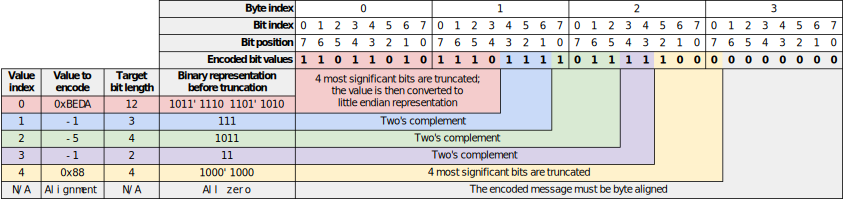
\includegraphics[width=\textwidth]{dsdl/bit-encoding}
	\caption{DSDL serialization example.\label{fig:dsdl_serialization_example}}
\end{figure}

\subsection{Scalar values}

The table \ref{table:dsdl_scalar_serialization} lists the scalar value serialization rules.

\begin{UAVCANSimpleTable}{Scalar value serialization}{|l l X|}\label{table:dsdl_scalar_serialization}
    Type                    & Bit length    & Binary format \\
    \texttt{bool}           & 1
                            & Single bit
                            \\
    \texttt{int\textbf{X}}  & X
                            & Two's complement signed integer
                            \\
    \texttt{uint\textbf{X}} & X
                            & Plain bits
                            \\
    \texttt{float16}        & 16
                            & IEEE 754 binary16
                            \\
    \texttt{float32}        & 32
                            & IEEE 754 binary32
                            \\
    \texttt{float64}        & 64
                            & IEEE 754 binary64
                            \\
    \texttt{void\textbf{X}} & X
                            & X zero bits; ignore when decoding
                            \\
\end{UAVCANSimpleTable}

\subsection{Nested data structures}

Nested data structures are serialized directly in-place,
as if their DSDL definition was pasted directly in place of their reference.
No additional prefixes, suffixes, or padding is provided.

\subsection{Fixed size arrays}

Fixed-size arrays are serialized as a plain sequence of items,
with each item serialized independently in place, with no alignment.
No extra data is added.

Essentially, a fixed-size array of size $X$ elements will be serialized exactly in the same way
as a sequence of $X$ fields of the same type in a row.
Hence, the following two data type definitions will have identical binary representation,
the only actual difference being their representation for the application
if automatic code generation is used.

\begin{minted}{python}
AnyType[3] array
\end{minted}

\begin{minted}{python}
AnyType item_0
AnyType item_1
AnyType item_2
\end{minted}

\subsection{Dynamic arrays}

The following two array definitions are equivalent;
the difference is their representation in the DSDL definition for better readability:
\begin{minted}{python}
AnyType[<42] a      # Can contain from 0 to 41 elements
AnyType[<=41] b     # Can contain from 0 to 41 elements
\end{minted}

A dynamic array is serialized as a sequence of serialized items prepended with an unsigned
integer field representing the number of contained items - the \emph{length field}.
The bit width of the length field is a function of the maximum number of items in the array:
$$\lceil{}\log_2 (X + 1)\rceil{}$$
where $X$ is the maximum number of items in the array.
For example, if the maximum number of items is 251, the length field bit width must be 8 bits;
if the maximum number of items is 1, the length field bit width will be just a single bit.

It is recommended to manually align dynamic arrays by prepending them with void fields
so that the first element is byte-aligned, as that enables more efficient serialization and
deserialization.
This recommendation does not need to be followed if the size of the array elements is not
a multiple of eight bits or if the array elements are of variable size themselves
(e.g., a dynamic array of nested types which contain dynamic arrays themselves).

Consider the following definition:

\begin{minted}{python}
void2                       # Padding - not required, provided as an example
AnyType[<42] array          # The length field is 6 bits wide (see the formula)
\end{minted}

If the array contained three elements,
the resulting binary representation would be equivalent to that of the following definition:

\begin{minted}{python}
void2                       # Padding - not required, provided as an example
uint6 array_length          # Set to 3, because the array contains three elements
AnyType item_0
AnyType item_1
AnyType item_2
\end{minted}

\subsection{Unions}

Similar to dynamic arrays, tagged unions are serialized as two subsequent entities:
the union tag followed by the selected field, with no additional data.

The union tag is an unsigned integer, the bit length of which is a function of the number of fields in the union:
$$\lceil{}\log_2 N\rceil{}$$
where N is the number of fields in the union.
The value serialized in the union tag is the index of the selected field.
Field indexes are assigned according to the order in which they are defined in DSDL,
starting from zero;
i.e. the first defined field has the index 0, the second defined field has the index 1, and so on.

Constants are not affected by the union tag.

It is recommended to manually align unions when they are nested into outer data types by
prepending them with void fields so that the elements are byte-aligned,
as that enables more efficient serialization and deserialization.

Consider the following example:

\begin{minted}{python}
@union                  # In this case, the union tag requires 2 bits
uint16  FOO = 42        # A regular constant attribute
uint16  a               # Index 0
uint8   b               # Index 1
float64 c               # Index 2
uint32  BAR = 42        # Another regular constant
\end{minted}

In order to encode the field \verb|b|, which, according to the definition,
has the data type \verb|uint8|, the union tag should be assigned the value 1.
The following structure will have an identical layout:

\begin{minted}{python}
uint2 tag               # Set to 1
uint8 b                 # The actual data
\end{minted}

If the value of \verb|b| was 7, the resulting serialized byte sequence would be (in binary):
$$%
\underbrace{\texttt{01}}_{\text{tag}}%
\overbrace{\texttt{000001 11}}^{\text{field }\texttt{b}}%
\underbrace{\texttt{000000}}_{\text{padding}}%
$$
